\documentclass[preprint,12pt]{elsarticle}

\usepackage{amsmath,amssymb}
\usepackage{booktabs}
\usepackage{graphicx}
\usepackage[hidelinks]{hyperref}

\journal{Journal Name}

\begin{document}

\begin{frontmatter}

\title{Selfrace: A Reinforcement Learning Framework for Autonomous Driving Simulation}

\author[inst1]{First Author}
\author[inst1]{Second Author}

\affiliation[inst1]{
  organization={Your University or Laboratory},
  addressline={Department or Institute},
  city={City},
  country={Country}
}

\begin{abstract}
This file is a ready-to-build Elsevier journal manuscript template based on
the \texttt{elsarticle} class. Replace this paragraph with a concise summary
of the research problem, method, main results, and implications.
\end{abstract}

\begin{keyword}
autonomous driving \sep reinforcement learning \sep simulation \sep decision making
\end{keyword}

\end{frontmatter}

\section{Introduction}

Autonomous driving research often depends on controllable simulation
environments for training and evaluation. This manuscript template can be used
as a starting point for a journal submission and already includes common
elements such as citations, equations, figures, and tables.

The source code for this project can be cited as supporting implementation
material. Replace this sentence with the contribution statement of the paper.

\section{Related Work}

Journal manuscripts usually summarize the closest lines of work and explain
how the proposed method differs from them. A citation example is shown here
\citep{sutton2018reinforcement}.

\section{Method}

Let $s_t$ denote the simulation state, $a_t$ the selected action, and $r_t$
the reward at time step $t$. A standard objective is
\begin{equation}
  J(\theta) = \mathbb{E}_{\pi_\theta}\left[\sum_{t=0}^{T}\gamma^t r_t\right],
\end{equation}
where $\gamma$ is the discount factor and $\pi_\theta$ is the policy.

\begin{figure}[t]
  \centering
  \IfFileExists{../images/network_architecture.png}{
    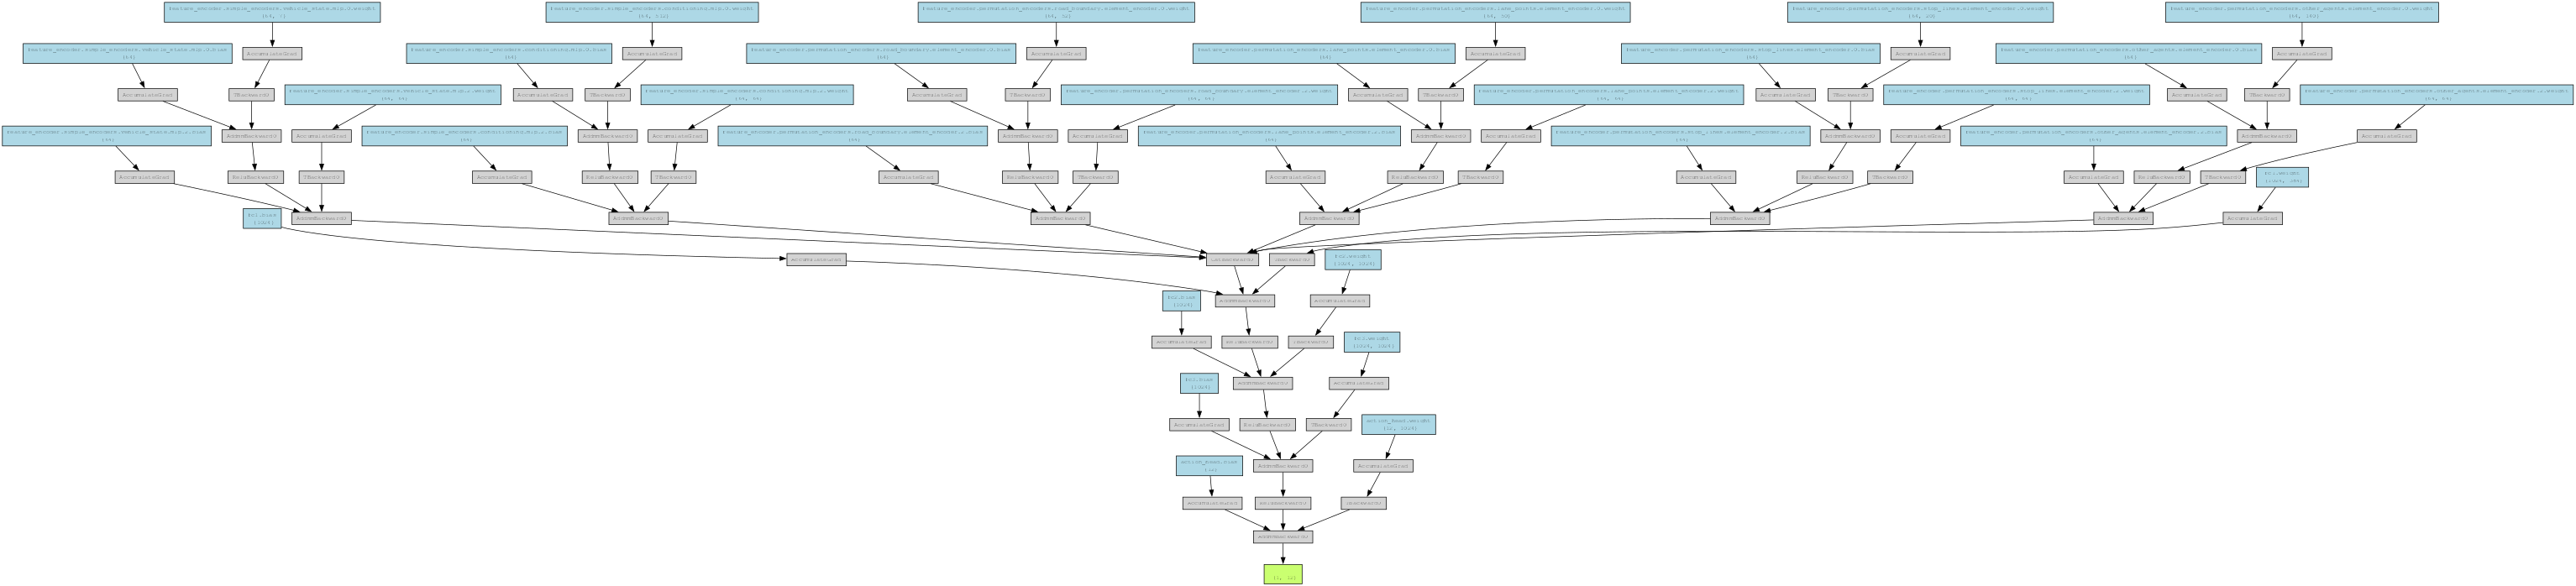
\includegraphics[width=0.78\linewidth]{../images/network_architecture.png}
  }{
    \fbox{\rule{0pt}{1.6in}\rule{0.78\linewidth}{0pt}}
  }
  \caption{Example figure placeholder. Replace it with the architecture or
  experiment diagram for the manuscript.}
  \label{fig:architecture}
\end{figure}

\section{Experiments}

Describe datasets, scenarios, baselines, metrics, hardware, and random seeds.
Table~\ref{tab:example-results} shows a compact result-table style.

\begin{table}[t]
  \centering
  \caption{Example experimental results. Replace the values with real metrics.}
  \label{tab:example-results}
  \begin{tabular}{lccc}
    \toprule
    Method & Success Rate & Collision Rate & Mean Reward \\
    \midrule
    Baseline & 0.72 & 0.18 & 124.3 \\
    Proposed & 0.86 & 0.09 & 168.7 \\
    \bottomrule
  \end{tabular}
\end{table}

\section{Conclusion}

Summarize the main findings, limitations, and future work. Keep this section
short and specific.

\section*{Declaration of Competing Interest}

The authors declare that they have no known competing financial interests or
personal relationships that could have appeared to influence the work reported
in this paper.

\section*{Data and Code Availability}

The code and data availability statement should be updated before submission.

\bibliographystyle{elsarticle-num}
\bibliography{references}

\end{document}
